\documentclass[a4paper, 12pt]{article}

\def\docname{Documentation Technique}

\usepackage{./common/preamble}
\def\dir{tech_documentation}

\begin{document}

\titlePage

\newpage

\resume{\dir}

\newpage

\docdescription{\dir}

\newpage

\tableofcontents

\newpage

\section{Organisation \& Communication}
\import{\dir}{orga.tex}

\section{Structure du projet}
\begin{figure}[H]
	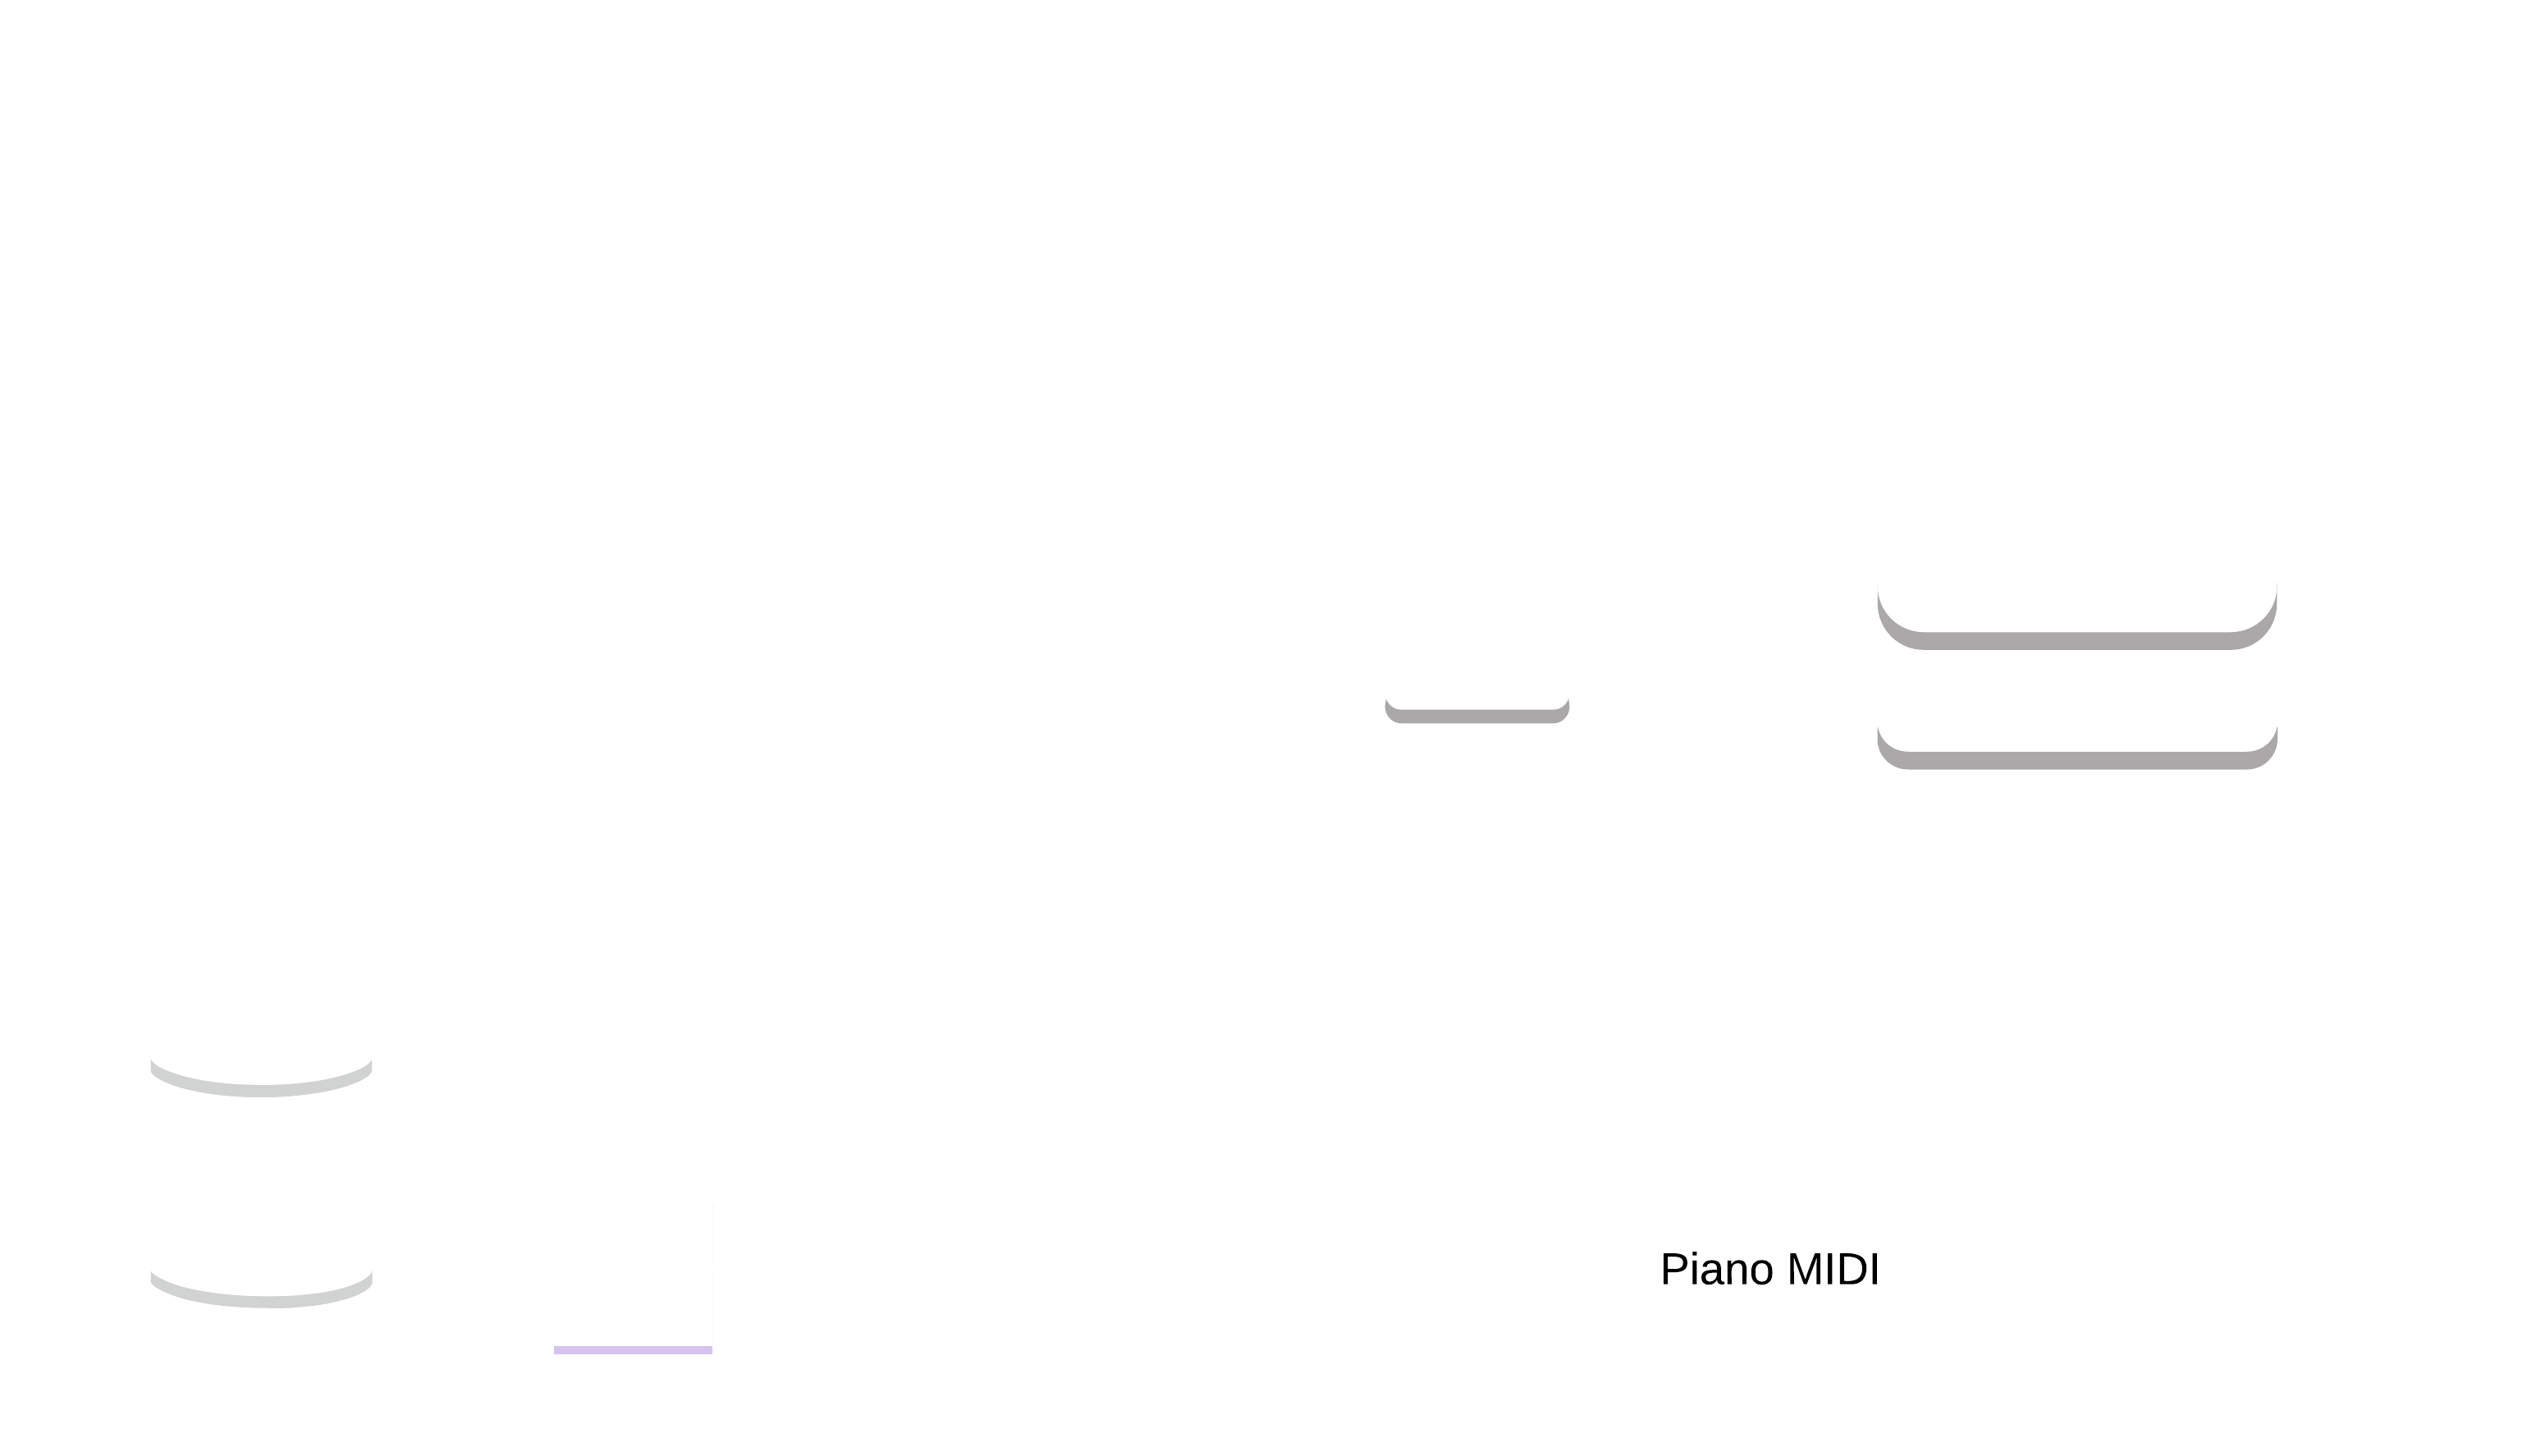
\includegraphics[width=\textwidth]{../assets/structure.png}
	\caption{Les composants du projet et leurs relations}
\end{figure}

La figure 1 illustre les differents composants du projet, ainsi que leurs relations

\begin{itemize}
	\item La base de données, accessible uniquement depuis le server. 
	\item Le server, qui puise et persiste les informations dans/avec la BDD.
	\item Le font, qui recupère les informations necessaires (authentication, catalogue, etc.) depuis le server. Il communique egalement avec le scorometer pour calculer en temps réel les scores
	\item Le Scorometer, qui donne en temps réel les scores, et les envoie au server pour les sauvegarder.
\end{itemize}

\section{Composants du projet}

\subsection{Base de données}
\import{\dir/db}{root.tex}

\subsection{Server}
\import{\dir}{server.tex}

\subsection{Scorometer}
\import{\dir}{scorometer.tex}

\subsection{Application Front-End}
\import{\dir}{front.tex}

\section{Norme}
\import{\dir}{norme.tex}

\section{Intégration Continue}
\import{\dir}{ci.tex}

\section{Environnement de développement}
\import{\dir}{dev.tex}

\end{document}
